\documentclass[letterpaper,11pt]{article}

\usepackage{fontspec}
\usepackage{xeCJK}
%\setCJKmainfont{SimSun} % 设置默认的中文字体为楷体
\usepackage{latexsym}
\usepackage[empty]{fullpage}
\usepackage{titlesec}
\usepackage{marvosym}
\usepackage[usenames,dvipsnames]{color}
\usepackage{verbatim}
\usepackage{enumitem}
\usepackage[hidelinks]{hyperref}
\usepackage{fancyhdr}
\usepackage[english]{babel}
\usepackage{tabularx}
\usepackage{fontawesome5}
\usepackage{multicol}
\usepackage{graphicx}
\setlength{\multicolsep}{-3.0pt}
\setlength{\columnsep}{-1pt}

\pagestyle{fancy}
\fancyhf{}
\fancyfoot{}
\renewcommand{\headrulewidth}{0pt}
\renewcommand{\footrulewidth}{0pt}

\addtolength{\oddsidemargin}{-0.6in}
\addtolength{\evensidemargin}{-0.5in}
\addtolength{\textwidth}{1.19in}
\addtolength{\topmargin}{-.8in}
\addtolength{\textheight}{1.4in}
\urlstyle{same}
\raggedbottom
\raggedright
\setlength{\tabcolsep}{0in}


\titleformat{\section}{
	\vspace{-4pt}\scshape\raggedright\large\bfseries
}{}{0em}{}[\color{black}\titlerule \vspace{-5pt}]

\newcommand{\resumeItem}[1]{	
	\item\small{
		{#1 \vspace{-2pt}}
	}
}

\newcommand{\classesList}[4]{
	\item\small{
		{#1 #2 #3 #4 \vspace{-2pt}}
	}
}

\newcommand{\resumeSubheading}[4]{
	\vspace{-2pt}\item
	\begin{tabular*}{1.0\textwidth}[t]{l@{\extracolsep{\fill}}r}
		\textbf{\CJKfamily{STSong}#1} & \textbf{\small #2} \\
		\textit{\small\CJKfamily{KaiTi}#3} & \textit{\small #4} \\
	\end{tabular*}\vspace{-7pt}
	
}

\newcommand{\resumeSubSubheading}[2]{
	\item
	\begin{tabular*}{0.97\textwidth}{l@{\extracolsep{\fill}}r}
		\textit{\small\CJKfamily{STSong}#1} & \textit{\small #2} \\
	\end{tabular*}\vspace{-7pt}
}

\newcommand{\resumeProjectHeading}[2]{
	\item
	\begin{tabular*}{1.001\textwidth}{l@{\extracolsep{\fill}}r}
		\small#1 & \textbf{\small #2}\\
	\end{tabular*}\vspace{-7pt}
}


\newcommand{\resumeSubItem}[1]{\resumeItem{#1}\vspace{-4pt}}
\renewcommand\labelitemi{$\vcenter{\hbox{\tiny$\bullet$}}$}
\renewcommand\labelitemii{$\vcenter{\hbox{\tiny$\bullet$}}$}

\newcommand{\resumeSubHeadingListStart}{\begin{itemize}[leftmargin=0.0in, label={}]}	
	\newcommand{\resumeSubHeadingListEnd}{\end{itemize}}

\newcommand{\resumeItemListStart}{\begin{itemize}}
	\newcommand{\resumeItemListEnd}{\end{itemize}\vspace{-5pt}}

\begin{document}
	\begin{flushleft}
		\begin{minipage}{0.6\textwidth}
			{\huge 顾\hspace{0.5em}睿} \\ 
			
			\vspace{14pt}
			 % faMars
			{\small \raisebox{-0.2\height}\faUser ~ 男/1998.01} \\
			{\small \raisebox{-0.2\height}\faPhone ~ +86 17802920798} \\
			{\small \raisebox{-0.2\height}\faEnvelope ~ npukujui11@gmail.com} \\
		\end{minipage}
		\hfill % 填充空白空间,将照片挤压到右侧
		\begin{minipage}{0.3\textwidth}
			\hspace*{3cm}
			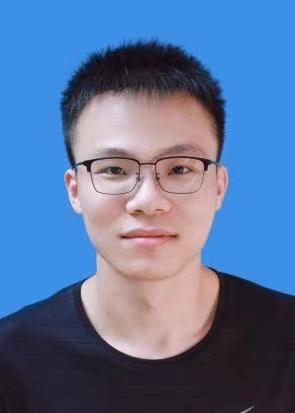
\includegraphics[width=0.4\textwidth]{picture/KuJui.jpg} % 替换为你的照片文件名
		\end{minipage}
		\vspace{-16pt}
	\end{flushleft}
	
	\section{教育经历}
	
	\resumeSubHeadingListStart
	\resumeSubheading
	{西北工业大学}{2015.09 -- 2019.06}
	{物联网工程}{本科,计算机学院}
	\vspace{-2pt}
	\resumeSubHeadingListEnd
	
	\resumeItemListStart
	\resumeItem{GPA \ 3.0/4.0 \ 【专业排名】\ 前40\%}
	\resumeItemListEnd
	
	\vspace{-8pt}
	
	\resumeSubHeadingListStart
	\resumeSubheading
	{兰州大学}{2022.09 -- 2025.06}
	{计算机科学与技术}{硕士,信息科学与工程学院}
	\vspace{-2pt}
	\resumeSubHeadingListEnd
	
	\resumeItemListStart	
	\resumeItem{GPA \ 3.8/4.0 \ 【专业排名】\ 前10\%}
	\resumeItemListEnd
	
	\vspace{-8pt}
	
	\section{专业技能\&荣誉奖励}

	\begin{itemize}[leftmargin=0in, label={}]
	\item{\textbf{专业技能:}{
			\vspace{-6pt}
			\begin{itemize}[leftmargin=0.15in]
				\small \item 熟练掌握计算机基础知识,本科阶段系统地学习了计算机组成原理、计算机网络、操作系统、数据库原理、嵌入式系统等理论课程。对物联网通信技术的原理和部署场景有一定的了解,如\textbf{Zigbee},\textbf{NB-IoT}等协议。
				\small \item
				了解\textbf{C/C\texttt{++}}语言的特性,能够熟练使用\textbf{智能指针}和\textbf{Valgrind}等工具来解决内存泄漏以及会使用相关的代码分析工具如\textbf{gprof}进行性能调优。此外熟练使用标准库如\textbf{STL}和第三方开源库\textbf{Boost}。
				\small \item 
				了解深度学习的原理和过程,熟悉使用\textbf{sckit-learn}等工具包以及熟悉\textbf{Tensorflow},\textbf{Pytorch}等深度学习架构的使用。
				\small \item 
				熟练使用\textbf{Git}和\textbf{SVN}等项目开发协作工具,具有基于嵌入式的软件开发能力,熟悉\textbf{A-SPICE}等软件开发流程。
			\end{itemize}}
		}
		
	\vspace{-8pt}
	
	\item{\textbf{证书 \& 获奖:}{
			\vspace{3pt}
			\begin{multicols}{2}
				\begin{itemize}[itemsep=-5pt, parsep=5pt]
					\small \item 英语(CET-4 520分);
					\small \item “工大出版社杯”数学建模二等奖;
					\small \item 校级优秀奖学金数次;
					\small \item 西工大校内 ACM 编程比赛二等奖;
					\small \item “电工杯”数学建模竞赛三等奖;
				\end{itemize}
			\end{multicols}}
		}		
			
	\vspace{-2pt}
	
	\item{\textbf{其他技能:}{
			\vspace{-6pt}
			\begin{itemize}[leftmargin=0.15in]
				\small \item 熟练使用\textbf{Office}办公软件,具有较强的总结和文档归纳能力,熟练使用\textbf{LaTex}和\textbf{Markdown}。
				\small \item 能够快速地学习新的知识体系,具有较强地团队协作能力和沟通交流能力。 
				\end{itemize}}
		}		
	\end{itemize}
	
	\section{工作实习\&项目经历}
	
	\resumeSubHeadingListStart

		\resumeSubheading
		{水下场景的多通道低光图像增强}{2023.06 -- 2024.07}	
		{硕士期间主要研究方向$|$ \emph{\textbf{Python, Deep Learning(VGG, ResNet, Transformer)}}}{ }
	
		\resumeItemListStart
			\resumeItem{基于\textbf{VGG}和\textbf{ResNet}现有模型改进,利用多卷积核对低光图像进行\textbf{HSV}通道分解,基于\textbf{U-Net}和\textbf{Transformer}结合基于 \textbf{CBAM} 改进的注意力机制构建不同通道之间弱光与真实值之间的非线性映射关系。}
			\resumeItem{基于我们改进的模型,解决了水下低光图像存在的亮度低、对比度差、图像质量低等问题,对于恢复图像的主要评价指标\textbf{PSNR}与\textbf{SSIM}接近\textbf{SOTA}指标的90\texttt{\%}。}
			\resumeItem{但针对于现阶段各类模型存在的大量残差连接所导致的访存次数增多,进而导致模型训练和推理效率变慢的问题,进行了优化,目前模型的\textbf{FLOPs}和\textbf{MACs}接近\textbf{SOTA}指标的80\texttt{\%}。}
		\resumeItemListEnd
		
		
		\resumeSubheading
		{基于UnityVR的晕动症激活系统}{2023.08 -- 2024.02}
		{硕士期间横向项目$|$ \emph{\textbf{C\texttt{\#}, Unity}}}{ }
		
		\resumeItemListStart
			\resumeItem{基于\textbf{Unity}游戏引擎和\textbf{Pico}平台,模拟一些真实场景,旨在通过PC端的蓝牙控制激发佩戴VR眼镜的实验者产生晕动症状(类似3D眩晕),为后续的晕动症脱敏训练提供实验支持。我们通过 \textbf{Unity Asset} 获取一些游戏模型、材质、插件等,如海面水系统,蓝牙插件等,加快Pico端的开发速度,并通过使用\textbf{C\texttt{\#}}编写脚本来控制游戏对象的行为和手柄输入.}
			\resumeItem{基于\textbf{WinForm}框架,结合第三方蓝牙库32feet实现一个Window程序,该程序通过串口蓝牙传输控制指令到VR设备以切换不同的场景。}
			\resumeItem{该项目为医学研究人员提供了一个有效的实验平台,提供了晕动症治疗和预防相关的的基础数据和技术支持。}
		\resumeItemListEnd
		% 这里要强调一些项目开发过程中遇到的问题以及我是如何解决的?比如如何优化应用的相应速度,如何处理大量数据的加载和现实,或者如何处理复杂的用户交互场景?以及控制协议的设置。
		% 详细讲解你在项目中使用的 WinForm 控件、设计模式(如 MVC/MVP)
		% 讲一下软件的模块化设置,如何确保系统的可维护性和可升级性。
		
		\resumeSubheading
		{汽车CVT软件开发工程师}{2019.07 -- 2021.08}
		{主要工作内容$|$ \emph{\textbf{C, A-SPICE, DOORS, EA, ASCET}}}{上汽通用五菱}
		
		\resumeItemListStart
		\resumeItem{主要参与\textbf{CVT}嵌入式控制软件架构的设计工作,并参与构建公司内部A-SPICE软件开发体系(涵盖使用需求管理工具\textbf{DOORS},系统设计工具\textbf{EA},开发和仿真工具\textbf{ASCET},主要负责开发规范,流程规范,文档设计规范,版本控制)。此外,个人负责整个软件中车辆驾驶模式识别模块与液压控制模块(占比15\texttt{\%})的软件功能实现和测试。}
		\resumeItem{项目涵盖的控制软件在离职时已基本完成系统测试与标定工作,在21年9月发布搭载该软件的2021款五菱星辰1.5T CVT,累计销量达7w台。2022年车质网发布的“2021年国内汽车投诉销量比排行榜”显示,该车型投诉销量比为\textbf{万分之0.2}排名榜单第一。}
		\resumeItemListEnd
	
		% 特地项目结束才主动离职选择考研,不想让别人说自己是害怕苦难就走了,有些考研的同事,选择提前离开。
	
		\resumeSubheading	
		{嵌入式软件开发实习生}{2018.07 -- 2018.09}
		{主要实习内容$|$ \emph{\textbf{C}}}{西安航空计算技术研究所}
		
		\resumeItemListStart
		\resumeItem{学习机载计算机处理器相关的CPU指令集(\textbf{MIPS、PowerPC})和CPU架构(\textbf{RISC、DSP})。结合部分模块的需求,使用\textbf{Protel}进行布局布线,并利用\textbf{Proteus}仿真工具验证设计,最终成功设计了一块4层的高速PCB,支持\textbf{SPI}和\textbf{I2C}接口。在实际测试中,该板子表现稳定,达到了预期的性能目标。}
		\resumeItem{负责了板子的主要设计工作,参与包括元器件选型、信号走线布局(主要解决信号完整和电磁兼容相关问题)以及信号完整性分析等工作。}
		\resumeItemListEnd
		
		
		% 使用了哪些工具和模拟器来实践这些指令集
		
		
		
		
		% DSP(数字信号处理器架构)
		% 学校安排的实习单位,很多都是涉密内容,当时不让拍照只让学习。631所主研方向和产品线主要是歼系列战斗机的飞控计算机。
		
		% 早期的歼7、歼8时代,一直采用分散式航空电子系统,每个系统都有自己的模拟式计算机。80年代,我国开始进行航空电子综合系统的研究,在歼-8B(02批)开始配备使用ARINC429总线的平显系统,并且首次通过和平典范计划引进了美国航空电子系统,首次采用了1553B总线,在与以色列的技术合作中我国首次接触以任务计算机为核心的多层多条总线为骨干的联合式航空电子系统,利用引进和自行研制的基础,我国完成了873航空电子系统的研制,该系统以任务计算机为核心,采用多条1553B数据总线,存储容量达到了1MB,将雷达、惯导、通信、大气数据计算机、外挂管理系统数据的集中处理与控制、信息的统一显示等功能,但由于当时我国尚没有大容量存储和高速光纤总线传输,与当时的先机水平仍有距离,我国的歼10、歼11、歼轰-7等战机都是在此基础上进行改进的。
		
		% ARINC 429 是一种广泛用于民用航空电子设备之间的数据通信标准。
		
		% MIL-STD-1553B 是一种广泛应用于军事和航空航天系统的串行数据总线标准。该标准最早由美国国防部在1973年发布,并在1978年发布了改进版 MIL-STD-1553B。该总线旨在实现机载系统中多个设备之间的可靠、抗干扰的数据传输。
		
		% MIL-STD-1553B 的关键特性
		% 双冗余设计:
		% MIL-STD-1553B 采用双冗余设计,即每个设备都通过两条总线连接,从而提高了系统的可靠性。如果其中一条总线出现故障,系统可以自动切换到另一条备用总线继续运行。
		
		% 半双工、差分信号:
		% 1553B 使用半双工通信方式,即在同一时间内只能进行发送或接收操作。它采用差分信号传输技术,通过减少电磁干扰(EMI)来提高通信的可靠性和抗干扰性。
		
		% 数据速率:
		% 1553B 总线的数据传输速率为 1 Mbps。虽然这个速率在今天看来不算高,但对于多数军事和航空应用中的控制和监控任务是足够的。
		
		% 时分多路复用:
		% 1553B 总线采用时分多路复用(TDM)技术,以便在一条总线上能够有多个设备进行通信。每个设备都有自己的时间片用于发送或接收数据,避免了总线冲突。
		
		% 命令/响应协议:
		% 1553B 总线使用命令/响应通信协议。总线控制器(BC)负责发送命令,然后遥测终端(RT)作出响应。这样可以有效管理总线通信并防止冲突。
		
		% 主从架构:
		% 总线控制器(Bus Controller, BC)是系统的主设备,负责管理总线通信,发送命令帧。遥测终端(Remote Terminal, RT)是从设备,响应来自 BC 的命令。还有一个总线监控器(Bus Monitor, BM),用于监视总线上发生的所有通信。
		
		% 873航电系统改进中,DTU部分处理器采用了有国内深圳某企业国产化的PACE1750A系列处理器(以MIL-STD-1750A指令集标准设计的处理器,MIL-STD-1750A是美国1980年初公布的一种军标,它详细定义了机载计算机的指令系统结构。),16位,主频30MHz,浮点运算DAIS MIX 1.3MIPS在指令集和数据混合使用下可寻址1MB字节,256KB RAM。
		
		
		% 现在第五代战斗机总线都采用光纤,数据传输速度10Gb/s 
	\resumeSubHeadingListEnd
	
	\vspace{-16pt}
	
	\section{本科学习经历}
	
	\resumeSubHeadingListStart
	
		\resumeSubheading	
		{基于智能手表的实时情绪感知与识别系统}{2018.09 -- 2019.04}
		{本科毕业设计$|$ \emph{\textbf{Python, Machine Learning}}}{}
		\resumeItemListStart
		\resumeItem{利用可穿戴设备采集人体数据(心率、皮肤电等),通过小波变换和快速傅里叶变换处理数据噪声去除噪声,使用\textbf{PCA}算法降维,并采用聚类算法进行预处理,并通过交叉验证优化模型参数,进而改进\textbf{SVM}模型提高情绪状态识别的准确性。}
		\resumeItem{采用了\textbf{AdaBoost}增强SVM模型的性能,对比改进前后的分类准确率从85\texttt{\%}提高到92\texttt{\%}}。
		\resumeItemListEnd

		\resumeSubheading	
		{红楼梦前八十回和后四十回作者异同分析}{2018.05}
		{“工大出版社杯”数学建模比赛$|$ \emph{\textbf{Python, Machine Learning}}}{}
		\resumeItemListStart
		\resumeItem{分析《红楼梦》前八十回与后四十回作者异同。主要通过\textbf{jieba}库对每章主要人物姓名的频率、虚词和主要单词的词频、词与词之间的相关性、段落字数词数进行特征提取,使用\textbf{sklearn}将文本数据转化为词频向量。随后采用\textbf{PCA}分析降维,并采用\textbf{K-Means}和\textbf{SVM}模型进行分析。}
		\resumeItemListEnd
		% 为什么主要人物的姓名频率、虚词和词语频率能代表作者的写作风格?为什么要研究词与词之间的相关性?
	
		\resumeSubheading	
		{微信智能家居控制中心}{2018.04 -- 2018.06}
		{物联网工程核心专业课程$|$ \emph{\textbf{PHP、ZigBee}}}{}
		\resumeItemListStart
		\resumeItem{利用\textbf{STM32}控制板通过\textbf{UART}串口结合改进的\textbf{ZigBee}协议栈,实现传感器、微信、云平台三方的连接,从而实现宿舍温湿度数据采集和控制。}
		% 如果需要,可以提到常见的控制板选项(如 Arduino、ESP8266、Raspberry Pi、STM32 等)和它们的特性,说明你选择控制板时考虑的因素,如处理能力、接口支持、功耗和成本。
		\resumeItemListEnd
		
		\resumeSubheading
		{简易计算机操作系统}{2017.09 -- 2018.01}
		{计算机操作系统课程$|$ \emph{\textbf{x86 汇编、C}}}{}
		\resumeItemListStart
		\resumeItem{构建了一个简易的计算机操作系统,涵盖操作系统的基本模块如引导加载(\textbf{x86汇编、Bootloader})、内存管理、文件系统、多任务处理、GUI和底层硬件交互(BIOS调用、中断处理)。}
		\resumeItem{基于\textbf{Haribote OS}的TCB数据结构和上下文切换方法,将原有的RR调度修改为优先级调度,实现了一个支持多任务调度的内核,能够同时处理5个并发任务。此外,优化了内存管理模块,一是从首次适配调整为最佳适配,二是额外增加了内存池管理,使得内存分配和回收的效率提升了近\texttt{20\%}}
		\resumeItemListEnd
	\resumeSubHeadingListEnd
	
	\vspace{-15pt}
	
	
\end{document} 